% ============================================================
% 交流回路（オシロスコープを用いた測定） 本文
% 原本: 実験手引書_交流回路(オシロスコープを用いた測定).docx（である調 → です・ます調に変更）
% 担当の先生はこのファイルと figures/ だけを編集してください。
% 図のラベルは fig:oscilloscope-○○ の形にしてください（他テーマとの重複防止）。
% ============================================================
\graphicspath{{contents/02_oscilloscope/figures/}}

\experimenttitle{交流回路（オシロスコープを用いた測定）}

% ============================================================
\section{目的}

オシロスコープの使い方を習得し，基本的なフィルタ回路の動作原理を理解します。

% ============================================================
\section{実用例（音源(PC)から高音成分を除去し，スピーカーから出る音で確認）}

フィルタ回路の1つにローパスフィルタがあります。この回路は高い周波数成分を遮断する機能を有するため，音楽などに含まれる高音成分を取り除くことが可能です。

% ============================================================
\section{原理}

% ------------------------------------------------------------
\subsection{交流}

交流（AC: Alternating Current）とは，時間経過とともに大きさと向きが周期的に変化するものです。典型的な交流波形を図\ref{fig:oscilloscope-waveforms}に示します。

\begin{figure}[htbp]
  \centering
  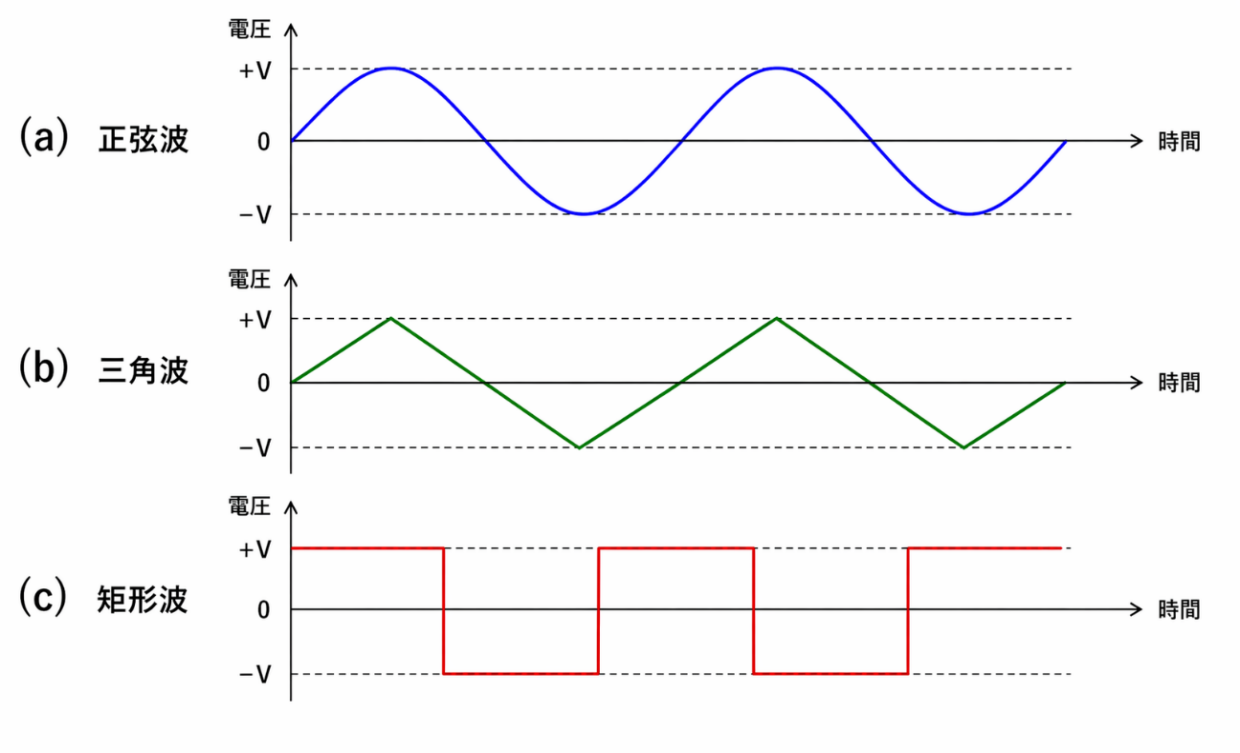
\includegraphics[width=0.7\linewidth]{oscilloscope_waveforms.png}
  \caption{交流波形の例}
  \label{fig:oscilloscope-waveforms}
\end{figure}

図\ref{fig:oscilloscope-waveforms}(a)は正弦波（sinusoidal wave），(b)は三角波（triangular wave），(c)は方形波（または矩形波）（rectangular wave）と呼ばれます。図\ref{fig:oscilloscope-waveforms}(a)のように電圧，電流の大きさが正弦波状に変化するものを正弦波交流といい，交流波形のなかでも最も基本となる波形です。

\begin{figure}[htbp]
  \centering
  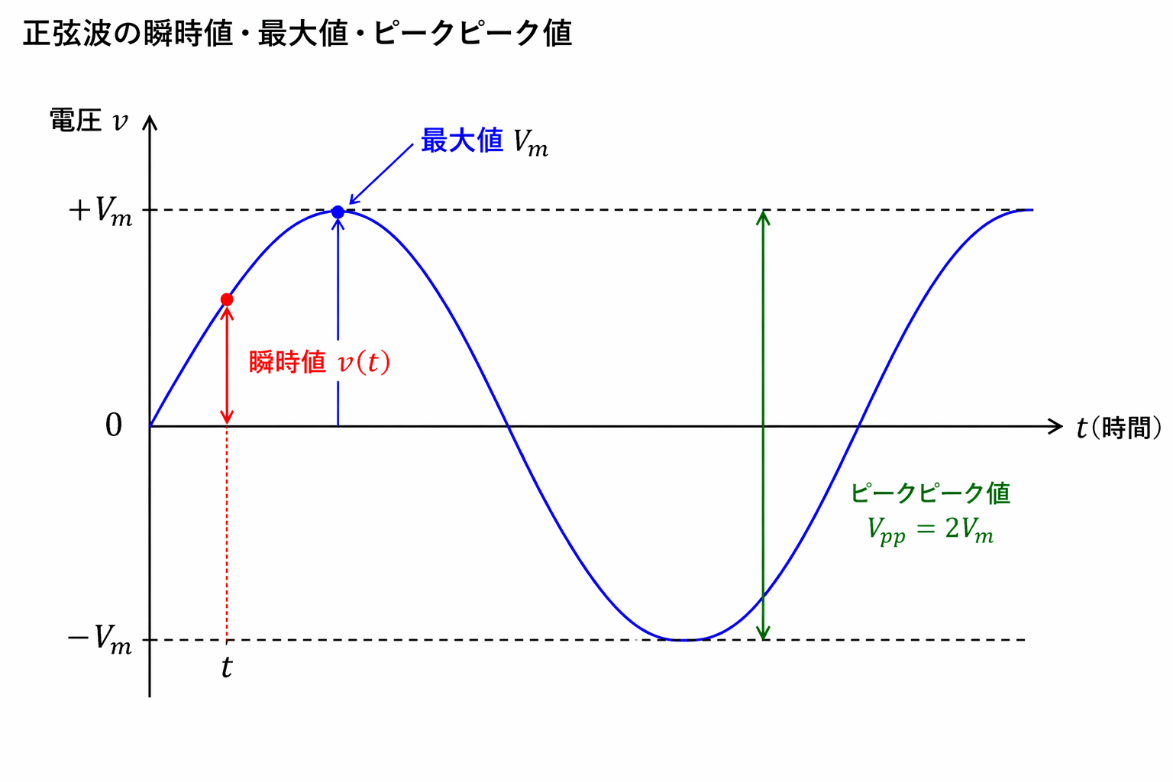
\includegraphics[width=0.7\linewidth]{oscilloscope_instantaneous.png}
  \caption{瞬時値と最大値}
  \label{fig:oscilloscope-instantaneous}
\end{figure}

図\ref{fig:oscilloscope-instantaneous}に示すように交流の任意の時間 $t$ における電圧・電流の値を「瞬時値（instantaneous value）」といいます。瞬時値は電圧の場合には $v$ と表され，電流の場合は $i$ で表されます。瞬時値のなかでも絶対値が最も大きいものを「最大値（maximum value）」といいます。最大値は電圧の場合は $V_\mathrm{m}$ で，電流の場合は $I_\mathrm{m}$ で表されます。最大値のことを「振幅（amplitude）」ともいいます。また，最大値と最小値の差を「ピークピーク値（peak-to-peak value）」といいます。ピークピーク値は電圧の場合 $V_\mathrm{pp}$，電流の場合 $I_\mathrm{pp}$ で表されます。交流の瞬時電圧は一般的にはオシロスコープ（oscilloscope）を用いて測定します。オシロスコープとは，電気信号（電圧）の時間経過に対する変動を測って波形として画面に表示して観測する測定器です。

% ------------------------------------------------------------
\subsection{$RC$回路（ローパスフィルタ）}

% TODO(原文確認): 見出し・本文は RC ローパスフィルタだが，図は LC ローパスフィルタ（原本のまま）
\begin{figure}[htbp]
  \centering
  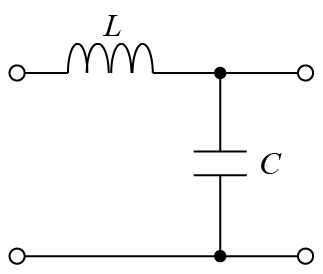
\includegraphics[width=0.35\linewidth]{oscilloscope_lc_lowpass.png}
  \caption{$LC$ローパスフィルタの回路図}
  \label{fig:oscilloscope-lc-lowpass}
\end{figure}

$RC$ローパスフィルタは，低い周波数は通して，高い周波数は通しにくくする回路です。$RC$ローパスフィルタは，抵抗（$R$）とコンデンサ（$C$）を組み合わせて構成されます。低い周波数成分を通し，高い周波数成分を減衰させる回路です。出力は一般的にコンデンサの両端から取り出されます。コンデンサは周波数が低いと電流を流しにくく，周波数が高いと電流を流しやすいという性質を持つため，低周波信号では出力電圧がほぼそのまま保持されます。一方，高周波信号では電流がコンデンサを通って接地側へ流れやすくなり，出力電圧が小さくなります。この性質により，高周波のノイズを除去し，滑らかな電圧波形を得ることができます。\important{周波数特性の境目となる周波数はカットオフ周波数と呼ばれ}，その値は
\begin{equation}
  f_\mathrm{c} = \frac{1}{2\pi RC}
  \label{eq:oscilloscope-cutoff}
\end{equation}
で表されます。$RC$ローパスフィルタは，ノイズ除去，平滑回路など電子回路やパワーエレクトロニクス分野で広く利用されています。

% ------------------------------------------------------------
\subsection{$RLC$直列共振フィルタ回路}

\begin{figure}[htbp]
  \centering
  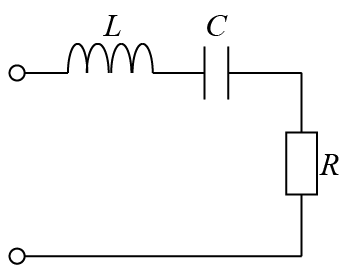
\includegraphics[width=0.35\linewidth]{oscilloscope_rlc_series.png}
  \caption{$RLC$直列共振の回路図}
  \label{fig:oscilloscope-rlc-series}
\end{figure}

交流回路では，抵抗は周波数が変化しても影響はありませんが，コイル $L$ やコンデンサ $C$ は周波数の変化に伴い，性質が変化します。コイルは周波数が高くなるほど電流を流しにくくなり，コンデンサは逆に周波数が高くなると電流を流しやすくなります。また，ある特定の周波数になると，コイルとコンデンサのリアクタンスが等しくなります。この状態を\important{共振}といい，\important{共振周波数} $f_0$ は
\begin{equation}
  f_0 = \frac{1}{2\pi\sqrt{LC}}
  \label{eq:oscilloscope-resonance}
\end{equation}
で表せます。

% ------------------------------------------------------------
\subsection{カットオフ周波数}

% 原文は「f_c = 1/√2 ≈ 0.707 となる周波数」。f_c の式ではなく出力電圧の比の意味なので書き換え（要確認）
カットオフ周波数 $f_\mathrm{c}$ とは，フィルタ回路が信号を通す領域と\important{減衰させる領域の境界となる周波数}です。一般的に，出力電圧が最大値の $1/\sqrt{2}\approx 0.707$ 倍となる周波数として定義されます（図\ref{fig:oscilloscope-lowpass-response}）。

\begin{figure}[htbp]
  \centering
  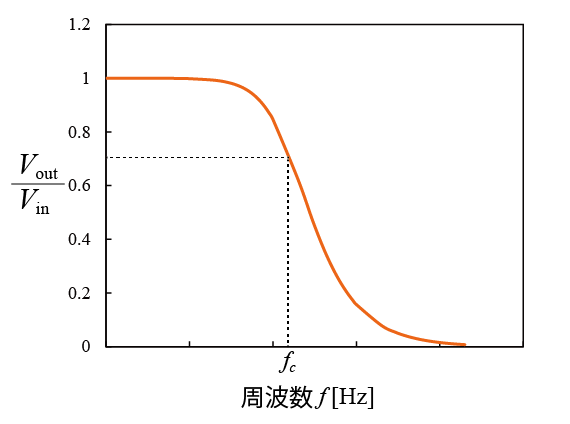
\includegraphics[width=0.5\linewidth]{oscilloscope_lowpass_response.png}
  \caption{ローパスフィルタの周波数特性}
  \label{fig:oscilloscope-lowpass-response}
\end{figure}

% ============================================================
\section{使用器具}

\begin{equipment}
\begin{itemize}
  \item オシロスコープ
  \item 交流電源（信号発生器）
  % TODO(原文確認): 実験2では 10 Ω の抵抗を使うが，ここには 100 Ω とある
  \item 抵抗（\SI{100}{\ohm}×1，\SI{1}{k\ohm}×1）
  \item コンデンサ（\SI{0.1}{\micro F}×1，\SI{1}{\micro F}×1）
  \item コイル（\SI{10}{mH}×1）
  \item ブレッドボード，ジャンパ線
\end{itemize}
\end{equipment}

% ============================================================
\section{実験方法}

測定結果は，ワークシートの表に記録してください。

% ------------------------------------------------------------
\subsection{実験1：$RC$ローパスフィルタの特性}

\begin{figure}[htbp]
  \centering
  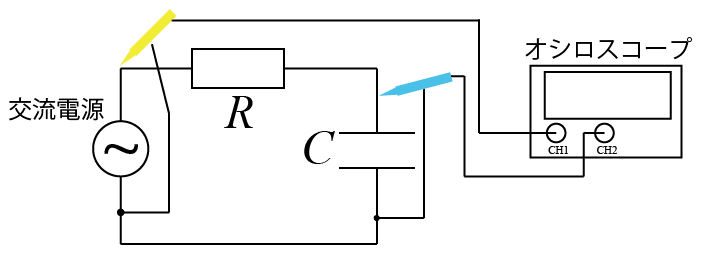
\includegraphics[width=0.75\linewidth]{oscilloscope_circuit1.png}
  \caption{測定回路1}
  \label{fig:oscilloscope-circuit1}
\end{figure}

\begin{procedure}[label=\textbf{1-\arabic*}, leftmargin=*, labelsep=0.8em]
  % 原文は「図4に示すような回路」だが測定回路1（図6）を指すと判断
  \item 図\ref{fig:oscilloscope-circuit1}に示すような回路を作製し，交流源（信号発生器）の周波数を変化させて出力電圧の最大値を測定します。ここで，交流電源の電圧を\SI{10}{V}に設定します。素子は抵抗\SI{1}{k\ohm}（茶黒赤金），コンデンサ\SI{1}{\micro F}を使用します。周波数は\SI{20}{Hz}～\SI{1}{kHz}まで変化させ，周波数特性を記録します。オシロスコープのCH1（黄）には入力波形，CH2（青）には出力波形を表示します。表示される波形の最大値 $V_\mathrm{m}$ を記録してください。\\
    ※Excelを用いてグラフを作成します。
  \item カットオフ周波数 $f_\mathrm{c}$ を確認します。
  \item 自作したローパスフィルタをPC（音源）とスピーカーに接続して機能を確認します。
\end{procedure}

% ------------------------------------------------------------
\subsection{実験2：$RLC$直列共振フィルタの特性}

\begin{figure}[htbp]
  \centering
  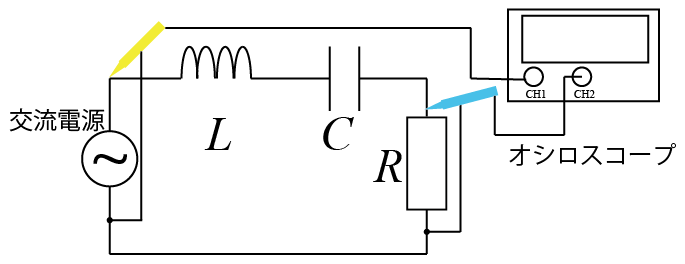
\includegraphics[width=0.75\linewidth]{oscilloscope_circuit2.png}
  \caption{測定回路2}
  \label{fig:oscilloscope-circuit2}
\end{figure}

\begin{procedure}[label=\textbf{2-\arabic*}, leftmargin=*, labelsep=0.8em]
  % 原文は「図5に示すような回路」だが測定回路2（図7）を指すと判断
  \item 図\ref{fig:oscilloscope-circuit2}に示すような回路を作製し，交流源（信号発生器）の周波数を変化させて出力電圧の最大値を測定します。ここで，交流電源の電圧を\SI{10}{V}に設定します。素子は抵抗\SI{10}{\ohm}（茶黒黒金），コイル\SI{10}{mH}，コンデンサ\SI{0.1}{\micro F}を使用します。周波数は\SI{2}{kHz}～\SI{8}{kHz}まで変化させ，周波数特性を記録します。オシロスコープのCH1（黄）には入力波形，CH2（青）には出力波形を表示します。CH2に表示される波形の最大値 $V_\mathrm{m}$ を記録してください。\\
    ※Excelを用いてグラフを作成します。
  \item 測定した結果から共振周波数を確認します。
\end{procedure}
